\section{Verification and controlled computational results}
\label{sec:experiments}

\subsection{Independent correctness checks}

The integrated repository suite passed \textbf{172 tests}, including all
134 baseline tests and 38 added Potts and integration tests.
The baseline and modified logs are both included. Their elapsed suite times
are not performance comparisons, since the modified suite performs additional
work.

The strongest cross-check constructs the entire normalized Jones Laurent
polynomial directly from each smoothing cube. It uses union--find on edge
labels, independent state-circle enumeration, and a separate quadratic
evaluation recurrence. It does not construct Tait graphs or use a frontier
transfer to obtain its expected answer.

\begin{table}[htbp]
\centering\small
\begin{tabularx}{\textwidth}{@{}Xr@{}}
\toprule
Independent or integration check & Completed count\\
\midrule
Validated diagrams in the full-polynomial oracle & 248\\
Complete smoothing states enumerated & 30,116\\
One-tensor exact color/shading/order comparisons & 4,464\\
Factored exact color/shading/order comparisons & 4,464\\
Additional weaving trace comparisons, each exact backend & 45\\
Adversarial direct labeled-spin comparisons with cancellations & 432\\
Residue annihilator and Fitting/Drazin identity cases & 524\\
Closed inverse-formula checks & 108\\
Radical-cutoff checks & 173\\
General-$p$ sharpness witnesses & 126\\
Nilpotent-residue companion witnesses & 18\\
Accepted certificate kinds in replay self-test & 2\\
Rejected tampered certificates & 21\\
\bottomrule
\end{tabularx}
\caption{Verification counts from the saved execution records. These finite
checks supplement the proofs; they do not replace them.}
\label{tab:checks}
\end{table}

The polynomial comparisons cover $q=5,6,7$, both checkerboard colors, and
natural, reversed and random crossing orders. Fixtures include Conway,
Kinoshita--Terasaka, a hard unknot, and connected sums. The additional
weaving comparisons extend to $m=49$, or 98 crossings.
Separate focused tests cover all 24 crossing orders of the figure-eight
diagram, mirrors, loops, parallel edges, orbit alignment cardinalities,
invalid options, deadline propagation and exact budget boundaries.

The radical-ring oracle uses exponent tuples rather than the production
packed binary algebra. Its 524 annihilator/Fitting cases include every
$2\times2$ matrix over $\F_2[x]/(x^2)$, a set of 256 matrices.
The sharpness checks vary $p,b,r$ and test both the surviving preceding
power and the first forced zero power. A separate finite-menu oracle checks
243 Laurent polynomials, 20 products of quadratic factors, and 5,151
writhe-dependent support intervals for Proposition~\ref{prop:menu}.

Finally, a real exact certificate for $W_{6001}$, with 12,002 crossings,
was serialized and replayed. Its largest coordinate had 21,791 bits.
The interpreter's decimal-conversion limit remained unchanged. This tests
the hexadecimal evidence format on actual large algebraic output; it is not
a new end-to-end recognition result for a short-braid family.

\subsection{Kernel benchmark design}

The principal timing record contains \textbf{3,045 timed calls}: 29 cases,
15 rounds and seven arms. The environment was Python 3.12.14 on Linux
6.18.44 with glibc 2.39. All raw nanosecond samples, arm orders,
inputs, crossing orders, counters and source hashes are included.
The corpus was specified as follows:
\begin{enumerate}
\item all 14 named JSON fixtures in the pinned implementation, with the
existing greedy order;
\item the first 12 accepted one-component five-strand, 16-crossing random
braid diagrams and their shuffled orders from seed 764259;
\item the three known five-color collision controls $W_5,W_7,W_{11}$.
\end{enumerate}
No random case was selected by its measured speedup.
The deliberately poor orders test representation sensitivity; they are not
claimed to approximate an input distribution in applications.

The seven arms are matching A1, modular $q=5$, factored modular $q=5$,
exact $q=5$, exact $q=6$, factored exact $q=6$, and matching A2.
The matching arms use the same modular $A$ as the five-color Potts
specialization. The exact six-color arms evaluate a different point and
have different collision behavior. They are valid cost comparisons, not
same-value numerical comparisons.

Each timed call receives the same supplied order and a fresh already
validated diagram object. Imports, input validation, order search and
diagram construction are outside the timed region. Tait extraction,
shading selection, transfer and normalization are inside it.
The counters and output values must reproduce exactly across repetitions.
Arm positions rotate between rounds to reduce systematic ordering effects.
The two identical matching arms provide an A/A noise control.

For each new arm, we report the median of the paired ratios
$T_{\mathrm{matching\ A1}}/T_{\mathrm{arm}}$. It need not equal the ratio
of the separately reported median times.
The saved order-statistic interval has nominal coverage at least 95 percent
under independent identically distributed rounds. Shared-machine timing
noise and dependence between rounds limit that interpretation; these are
descriptive intervals, not universal performance guarantees.
A local faster/slower label additionally requires the median ratio to lie
beyond the corresponding A/A interquartile range.
No multiple-comparison or population-level conclusion is drawn.

\subsection{Measured improvements and regressions}

% Generated by make_paper_figures.py; do not edit values by hand.
\begin{table}[htbp]
\centering
\footnotesize
\setlength{\tabcolsep}{3.5pt}
\begin{tabular*}{\linewidth}{@{\extracolsep{\fill}}lrrrrrrrr@{}}
\toprule
Input & $n$ & $w$ & $f$ & $g$ & $K_E$ & $K_F$ & $T_M/T_E$ & $T_M/T_F$ \\
\midrule
Conway & 11 & 6 & 3 & 3 & 5 & 6 & $1.574^{\dagger}$ & 1.298 \\
Kinoshita--Terasaka & 11 & 6 & 3 & 3 & 5 & 6 & $1.286^{\dagger}$ & 1.048 \\
Conway \#8 & 88 & 6 & 3 & 3 & 5 & 6 & $1.704^{\dagger}$ & 1.215 \\
Random 04 & 16 & 22 & 8 & 7 & 4,111 & 317 & $0.118^{\dagger}$ & $0.376^{\dagger}$ \\
Random 05 & 16 & 26 & 8 & 6 & 4,111 & 205 & $0.083^{\dagger}$ & $2.054^{\dagger}$ \\
Random 11 & 16 & 22 & 4 & 4 & 15 & 15 & $11.220^{\dagger}$ & $11.855^{\dagger}$ \\
\bottomrule
\end{tabular*}
\par\smallskip
\begin{minipage}{\linewidth}\scriptsize
$M$: matching kernel at the five-color evaluation point; $E$: exact $q=6$;
$F$: factored exact $q=6$. $K_E,K_F$ count peak represented keys; $K_F$
sums represented component tables. $f$ is the full active spin frontier
and $g$ the largest active frontier of one processed component.
Ratios are paired medians; values above one favor the denominator.
$\dagger$ marks a comparison meeting both the pointwise interval and A/A rule.
\end{minipage}
\caption{Selected supplied-order kernel results. The companion CSV retains all 29 cases, including every measured regression.}
\label{tab:kernel-selected}
\end{table}


The clearest factorization result is \code{random\_order\_05}.
The exact one-tensor implementation reaches 4,111 represented keys and
30,197 transitions. Its factored counterpart reaches 205 total represented
keys, at most 203 in one component, and 1,558 transitions.
The maximum global active-face count is eight and the maximum
component frontier is six. These discrete counts reproduce independently
of timing noise.

On this input, the paired one-tensor/factored exact median ratio is
$23.843$, with recorded interval $[19.448,29.683]$.
The same-specialization comparison is the strongest evidence for the
component optimization. Against the matching arm, factored exact $q=6$
has median ratio $2.054$ and interval $[1.878,2.552]$.

The negative control \code{random\_order\_04} is equally informative.
Factorization improves its own exact backend by a median factor of
$3.186$, yet its ratio against matching is only $0.376$:
matching remains substantially faster. Several other arbitrary orders
also favor matching. The factorized $q=6$ arm has five locally faster
cases, nine slower cases and fifteen without a clear timing claim under
the recorded rule. The one-tensor exact $q=6$ arm has eight, eight and
thirteen, respectively.

\begin{figure}[p]
\centering
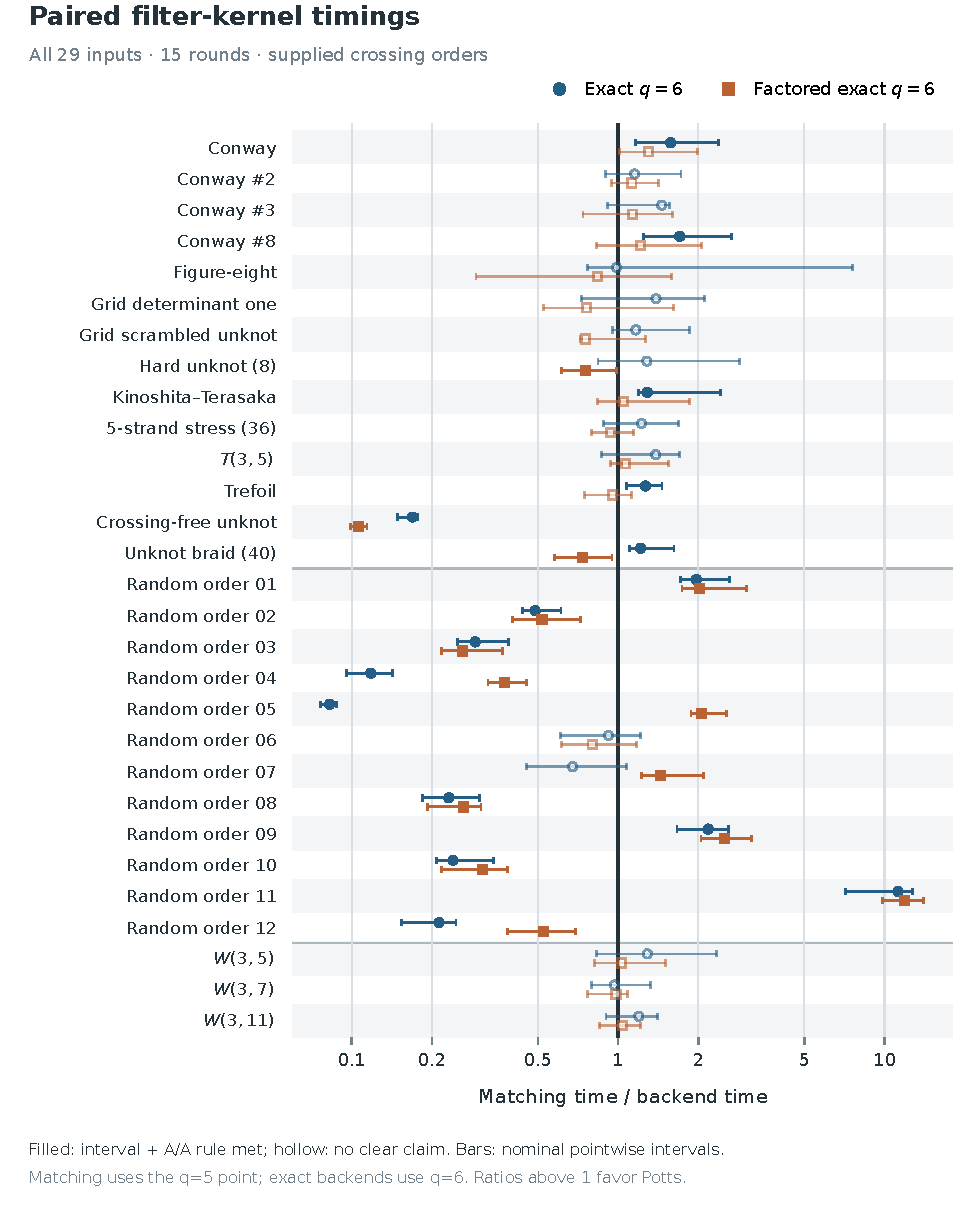
\includegraphics[width=\textwidth,height=0.87\textheight,keepaspectratio]{figures/kernel_ratios.pdf}
\caption{All 29 kernel comparisons against the same modular matching
reference. Ratios above one favor the indicated Potts arm. Exact $q=6$
uses a different Jones point from the modular reference. Intervals and
claim markers follow the recorded paired/A/A rule; regressions are shown
alongside improvements.}
\label{fig:ratios}
\end{figure}

\begin{figure}[htbp]
\centering
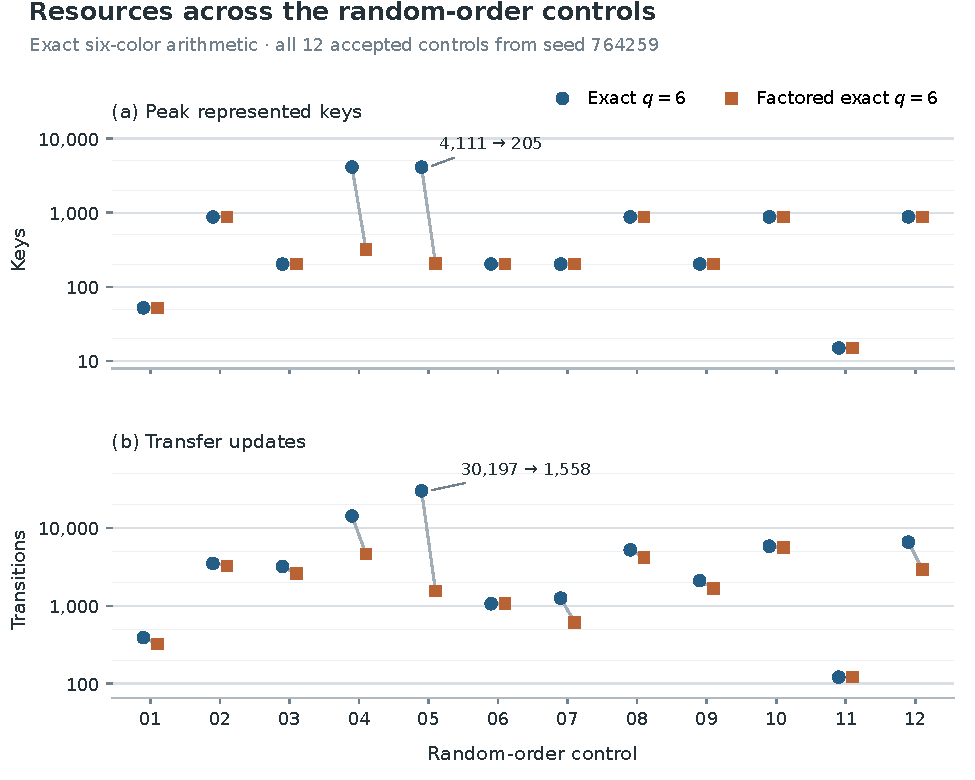
\includegraphics[width=\textwidth]{figures/component_resources.pdf}
\caption{Logical state and transition counts on all twelve fixed random-order
controls. These deterministic measures expose both the savings from
component independence and cases where little factorization is available.
State counts are not process-memory measurements.}
\label{fig:resources}
\end{figure}

Several larger named fixtures show favorable kernel medians, but many
intervals and A/A ranges are too wide to support a local claim for a
particular arm. These cases are retained without upgrading the evidence.
The examples establish that the representation can improve practical
work; they do not establish a growing-family runtime exponent.

\subsection{Normal-pipeline experiment}

A separate experiment contains \textbf{476 timed calls}: 17 inputs,
seven rotated rounds, matching A/A controls, exact $q=6$, and factored
exact $q=6$. It includes JSON parsing, validating diagram construction,
normal recognition and JSON output encoding. Imports, file I/O, CLI
parsing and process startup are excluded.
The matching backend uses its native generic $A$, and every ordinary
early stage remains enabled.

All verdicts are complete and consistent. Only five cases reach Jones:
Conway, Kinoshita--Terasaka, and Conway connected sums with two, three
and eight summands. The other twelve are decided earlier, including all
three weaving controls.

% Generated by make_paper_figures.py; do not edit values by hand.
\begin{table}[htbp]
\centering
\footnotesize
\setlength{\tabcolsep}{3.5pt}
\begin{tabular*}{\linewidth}{@{\extracolsep{\fill}}lrccc@{}}
\toprule
Input & $n$ & $T_M/T_E$ [interval] & $T_M/T_F$ [interval] & Supported claim \\
\midrule
Conway & 11 & 0.991 [0.448, 3.221] & 1.717 [0.605, 3.925] & None \\
Conway \#2 & 22 & 1.175 [0.582, 4.046] & 1.159 [0.286, 4.324] & None \\
Conway \#3 & 33 & 1.202 [0.292, 2.032] & 0.873 [0.426, 2.014] & None \\
Conway \#8 & 88 & 1.645 [0.474, 4.439] & 0.906 [0.346, 1.539] & None \\
Kinoshita--Terasaka & 11 & 1.374 [0.435, 3.422] & 1.973 [0.305, 3.946] & None \\
\bottomrule
\end{tabular*}
\par\smallskip
\begin{minipage}{\linewidth}\scriptsize
$M$: the normal pipeline with its native generic matching evaluation;
$E,F$: the normal pipeline with exact or factored exact $q=6$.
Nominal pointwise intervals; see the experimental-design assumptions in the text.
All five inputs reached Jones evaluation; the other twelve inputs bypassed it.
No comparison in this seven-round pipeline run met the timing-claim rule.
\end{minipage}
\caption{The five normal-pipeline cases that exercised the selected Jones backend. Timings include input parsing, checked diagram conversion, recognition, and JSON output encoding in a hot process.}
\label{tab:pipeline-selected}
\end{table}


\textbf{No full-pipeline speedup is supported by this seven-round run.}
The five cases that exercise Jones have wide intervals or A/A variation.
Backend speed claims are explicitly suppressed on bypassed cases.
This result limits the practical conclusion without weakening the proved
transfer bounds or the deterministic resource savings.

\subsection{Provenance and reproducibility limits}

The kernel source hashes agree before and after its timing run.
Subsequent edits changed only exact obstruction serialization wrappers and
added their shared helper; every raw evaluator and helper used in the
kernel timing has unchanged AST content. The exact measured versions of
all eight relevant modules were reconstructed and checked against the
recorded complete-file SHA-256 hashes. They are included as a provenance
snapshot, with the wrapper-only patch and audit record.
The normal-pipeline measurement uses the final wrappers and integrated
backends, with its own matching before/after hashes.

The corpus is small and timings are machine-dependent. Default budgets
were raised consistently for the kernel experiment to avoid comparing
early exits; all completed results and detection outcomes were checked.
There is no evidence here that a single representation dominates every
diagram, that an adaptive policy has already been validated, or that the
general recognizer has become quasi-polynomial.
